\chapter{Introdução}
\label{capitulo:introducao}

O projeto propõe o desenvolvimento de um novo módulo, no Sistema SLAB, o Teste de Tukey, uma ferramenta estatística essencial, que é amplamente utilizada para comparar múltiplas médias, tornando-se valioso em investigações científicas e aplicações práticas. Este documento descreve o projeto de implementação do Teste de Tukey em uma plataforma educacional e prática denominada SLAB. Embora o Slab seja uma fonte abrangente de conceitos estatísticos, ele não incluiu, até o momento, uma funcionalidade para calcular o Teste de Tukey. Portanto, o objetivo deste projeto foi introduzir essa funcionalidade, tornando o Statistical Lab uma ferramenta mais completa e versátil para análise estatística.

\chapter{Requisitos}

\subsection{Requisitos Não Funcionais}

%Será que preciso mesmo disso?
\requisitoNaoFuncional{RNF1}{O sistema deve ser feito na linguagem PHP}
{Joao Victor}{30 de outubro de 2023}{IF Goiano Ceres}
{Ronneesley Moura Teles}{rnf:linguagem}
{O sistema foi implementado na linguagem PHP, dessa forma o sistema de Tukey foi desenvolvida em PHP}

\requisitoNaoFuncional{RNF2}{O sistema deve ser portável}
{Joao Victor}{30 de outubro de 2023}{IF Goiano Ceres}
{Ronneesley Moura Teles}{rnf:portável}
{O sistema deve ser compatível com os principais navegadores da web, como Chrome, Firefox, e Edge.}

\requisitoNaoFuncional{RNF3}{O sistema deve funcionar na Web}
{Dr. Fulano de Tal}{30 de outubro de 2023}{IF Goiano Ceres}
{Ronneesley Moura Teles}{rnf:web}
{O sistema deve ser acessível via navegador Web}

\requisitoNaoFuncional{RNF4}{A interface do usuário deve ser feita em HTML e CSS.}
{Joao Victor}{30 de outubro de 2023}{IF Goiano Ceres}
{Ronneesley Moura Teles}{rnf:interface}
{A interface do usuário (HTML/CSS) deve ser amigável e intuitiva, guiando o usuário por todas as etapas do processo.}

\requisitoNaoFuncional{RNF5}{O sistema deve passar no teste}
{Joao Victor}{30 de outubro de 2023}{IF Goiano Ceres}
{Ronneesley Moura Teles}{rnf:teste}
{O sistema deve ser testado com testes unitários usando o framework PHPUnit para garantir a corretude do software.}

\requisitoNaoFuncional{RNF6}{O sistema deve ter uma documentação adequada.}
{Joao Victor}{30 de outubro de 2023}{IF Goiano Ceres}
{Ronneesley Moura Teles}{rnf:documentação}
{Deve haver documentação adequada do sistema, incluindo um manual do usuário e informações técnicas para desenvolvedores.}


\subsection{Requisitos Funcionais}

\requisito{RF1}{Inserir Dados}
{Joao Victor}{30 de outubro de 2023}{IF Goiano Ceres}
{Ronneesley Moura Teles}{Teste}{ Médias, q ,QMRes, r}
{O sistema deve permitir que o usuário insira valores de médias e ouutros parâmetros necessários para o teste de Tukey. Deve haver validações para garantir que os dados inseridos sejam numéricos e válidos.}

\requisito{RF2}{Executar Teste}
{Joao Victor}{30 de outubro de 2023}{IF Goiano Ceres}
{Ronneesley Moura Teles}{}{calcular(medias, q, qmRes, r)}
{O sistema deve calcular o teste de Tukey com base nos dados inseridos pelo usuário.
Deve-se garantir que os cálculos sejam precisos e corretos de acordo com as fórmulas estatísticas.}

\requisito{RF3}{Exibir Resultados}
{Joao Victor}{30 de outubro de 2023}{IF Goiano Ceres}
{Ronneesley Moura Teles}{Teste}{calcularDelta(q, qmRes, r)}
{O sistema deve apresentar os resultados do teste de Tukey, incluindo os grupos com diferenças significativas.
Deve fornecer informações estatísticas detalhadas para análise.}

\requisito{RF4}{Exibir Tabela com Resultado}
{Joao Victor}{30 de outubro de 2023}{IF Goiano Ceres}
{Ronneesley Moura Teles}{Teste}{classificar(mediasO, delta)}
{O sistema deve gerar representação por meio de tabela desenvolvida para ajudar na visualização das diferenças significativas e nas comparações estatísticas entre grupos.}

\chapter{Caso de Uso}

\casoUsoDetalhadoTextual{UC1}{Inserir dados do Teste de Tukey.}
{Usuário}
{Usuário: o usuário deseja inserir os dados para realizar o cálculo do teste de Tukey.}
{Nenhuma}
{O usuário tem a capacidade de inserir os dados necessários para realizar o Teste de Tukey no sistema.}
{
	\begin{enumerate}[label=FB\arabic*.]
		
		\item Entrar no Slab;
		\item Ir até a aba de Cálculos e localizar a aba Teste de Tukey;
		\item Entrar na aba Teste de Tukey;
		\item Usuario inserir as medias, qrest, numero de tratamentos e numero de repetição;
		
	\end{enumerate}
}{
	\begin{enumerate}[label=FA\arabic*.]
		\item Se o usuario não fornecer os valores corretos:
			\begin{enumerate}
				\item Osistema deve alertar e apontar onde esta o erro.
			\end{enumerate}
	\end{enumerate}
}{}{}

\casoUsoDetalhadoTextual{UC2}{Analisar Teste de Tukey.}
{Usuário}
{Usuário: O usuário pode solicitar que o sistema execute o Teste de Tukey com base nos dados fornecidos.}
{Nenhuma}
{O usuário solicita e o sistema executa o Teste.}
{
	\begin{enumerate}[label=FB\arabic*.]
	
		\item Depois de inserir os valores pedir para calcular.
		\item Analisar os cálculos.
		\item Usuario ddeterminar a relevancia do seu teste.
		\item Usuaria pode exportar os dados em csv.
		
	\end{enumerate}
}{
	\begin{enumerate}[label=FA\arabic*.]
		\item Se os valores não forem corretos:
			\begin{enumerate}
				\item O sistema volta para a tela Teste de Tukey.
			\end{enumerate}
	\end{enumerate}
}{}{}


\casoUsoDetalhadoTextual{UC5}{Realizar Teste de Tukey}
{Sistema}
{Sistema: O sistema é capaz de executar o Teste de Tukey com base nos dados fornecidos pelos usuários.}
{Nenhuma}
{O sistema executa o Teste de Tukey.}
{
	\begin{enumerate}[label=FB\arabic*.]
		\item O usuario deve fornecer os dados;
		\item O sistema executa o Teste.
		
	\end{enumerate}
}{
	\begin{enumerate}[label=FA\arabic*.]
		\item Se tiver dados incompletos
			\begin{enumerate}
				\item O sistema deve apontar o erro;
			\end{enumerate}
	\end{enumerate}
}{}{}

\casoUsoDetalhadoTextual{UC6}{Executar Teste}
{Sistema}
{Sistema: Uma ação interna do sistema que realiza o processamento estatístico necessário para conduzir o Teste de Tukey com base nos dados inseridos pelos usuários.}
{Nenhuma}
{O sistema realiza o processamento.}
{
	\begin{enumerate}[label=FB\arabic*.]
		\item O sistema processa os dados.
	
	\end{enumerate}
}{
	\begin{enumerate}[label=FA\arabic*.]
		\item Se houver algum erro:
			\begin{enumerate}
				\item O sistema deve apontar o erro.
			\end{enumerate}
	\end{enumerate}
}{}{}

\casoUsoDetalhadoTextual{UC7}{Exibir Tabela com Resultados de significância}
{Sistema}
{Sistema: Após a execução do teste, o sistema apresenta os resultados de significância de maneira tabular, fornecendo aos usuários uma visão clara das diferenças estatisticamente significativas entre os grupos.
}
{Nenhuma}
{O sistema apresenta os resusultados de significância corretamente.}
{
	\begin{enumerate}[label=FB\arabic*.]
		\item O sistema exibe a tabela com os resultados de significãncia;
		\item O usuario deve saber interpretar os resultados.
	\end{enumerate}
}{
	\begin{enumerate}[label=FA\arabic*.]
		\item Se houver erros:
			\begin{enumerate}
				\item O sistema deve apontar o erro;
				\item O usuario deve tentar compreender melhor sobre o teste de Tukey.
			\end{enumerate}
	\end{enumerate}
}{}{}

\begin{figure}[H]
  \centering
  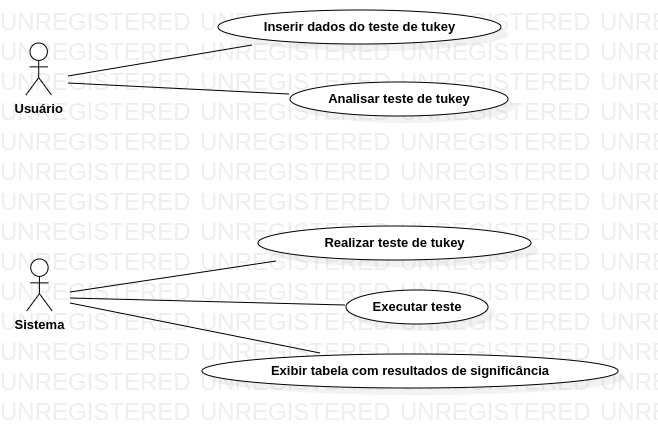
\includegraphics[width=0.8\linewidth]{imagens/casodeuso.png} 
  \caption{Diagrama Caso de Uso}
  \label{fig:exemplo}
\end{figure}

\chapter{Classes do Sistema}
\begin{tikzpicture}
  % Definindo as classes
  \begin{class}[text width=11cm]{TesteTukey}{0,0}
    \attribute{- delta: float}
    \attribute{- classes: array}
    \attribute{- indices:: array}
    \attribute{- mediasOrdenadas: array}
    \attribute{- nTratamentos: int}
    \attribute{- nClasses: int}
    \operation{ + temClasse(iO: int, nC: int): bool} 
	\operation{ + getNomeClasse(nC: int): string}
	\operation{ + calcular(medias: array, q: float, qmRes: float, r: int): void}
	\operation{ + calcularDelta(q: float, qmRes: float, r: int): float}
	\operation{ + classificar(mediasO: array, delta:  float): array}    	    	
	\operation{ + getDelta(): float}
	\operation{ + setDelta(delta: float): void}
	\operation{ + getClasses(): array}
	\operation{ + setClasses(classes: array): void}
	\operation{ + getMediasOrdenadas(): array}
	\operation{ + setMediasOrdenadas(mediasOrdenadas: array): void}
	\operation{ + getNTratamentos(): int}
	\operation{ + setNTratamentos(nTratamentos: int): void}                 	
	\operation{ + getNClasses(): int}
	\operation{ + setNClasses(nClasses: int): void}

  \end{class}

  \begin{class}[text width=5cm]{TesteTukeyControler}{0,-17}
    \attribute {- atributos e métodos herdados de ControleBase}
	\operation {+ processar(acao: string): void}        	
	\operation {+ mostrarConfiguracaoInicial(): void}   	
	\operation {+ calcular(): void}

  \end{class}

  % Relacionamento entre as classes
  \draw[umlcd style, ->] (TesteTukeyControler) -- (TesteTukey) node[midway,above]{$1..*$};

\end{tikzpicture}

\begin{figure}[H]
  \centering
  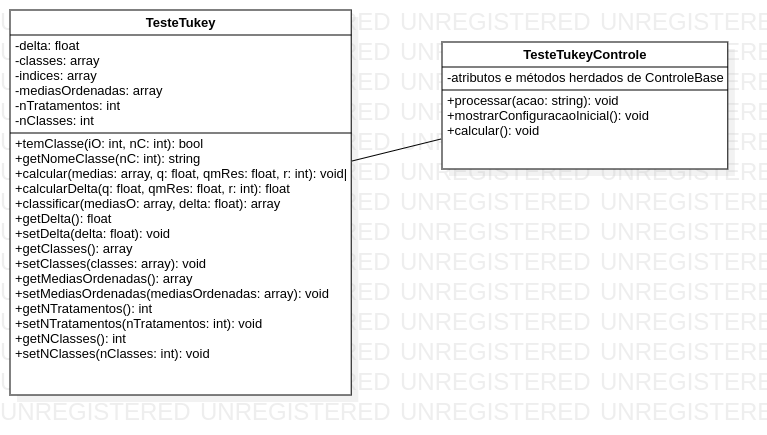
\includegraphics[width=0.8\linewidth]{imagens/classes.png} 
  \caption{Diagrama de Classe}
  \label{fig:exemplo}
\end{figure}

\chapter{Protótipos do sistema}


\begin{figure}[H]
  \centering
  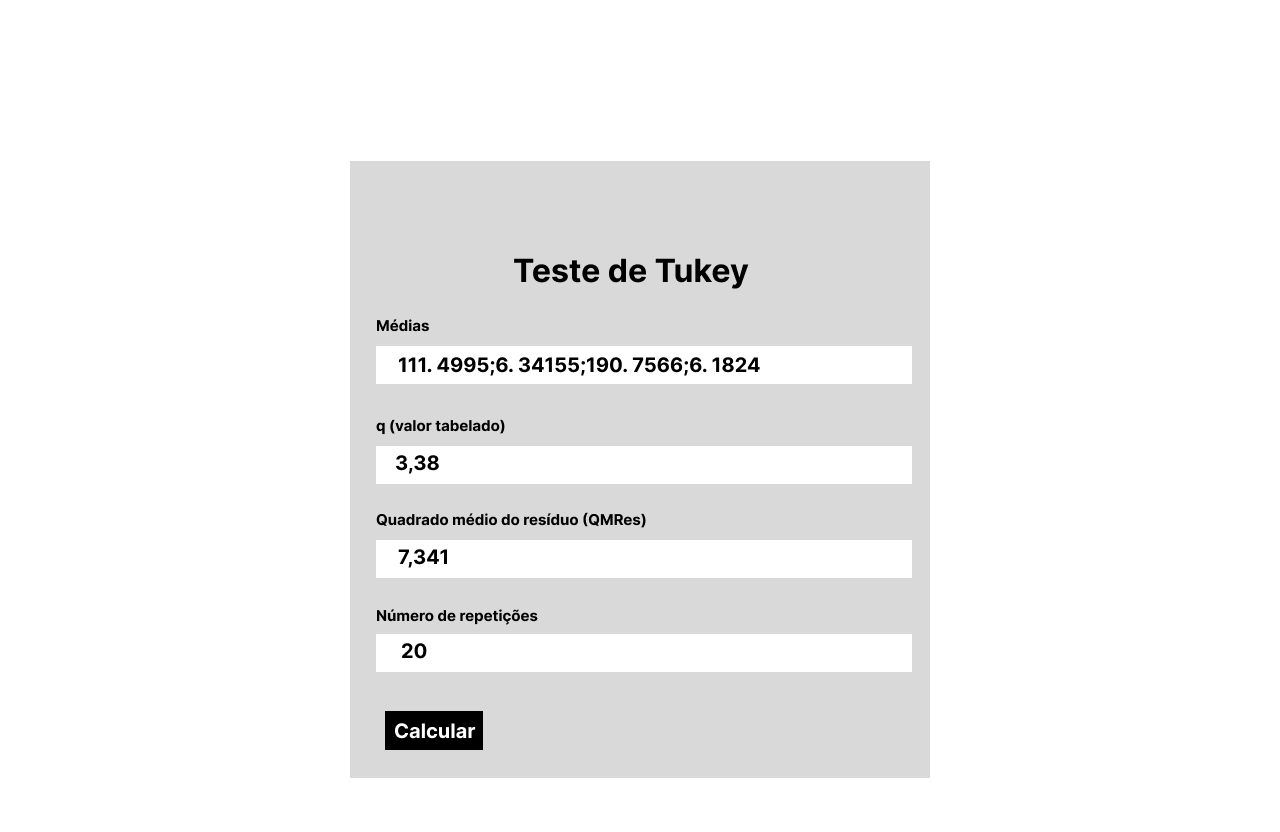
\includegraphics[width=0.8\linewidth]{imagens/tela1.png} 
  \caption{Tela Teste de Tukey}
  \label{fig:exemplo}
\end{figure}

\begin{figure}[H]
  \centering
  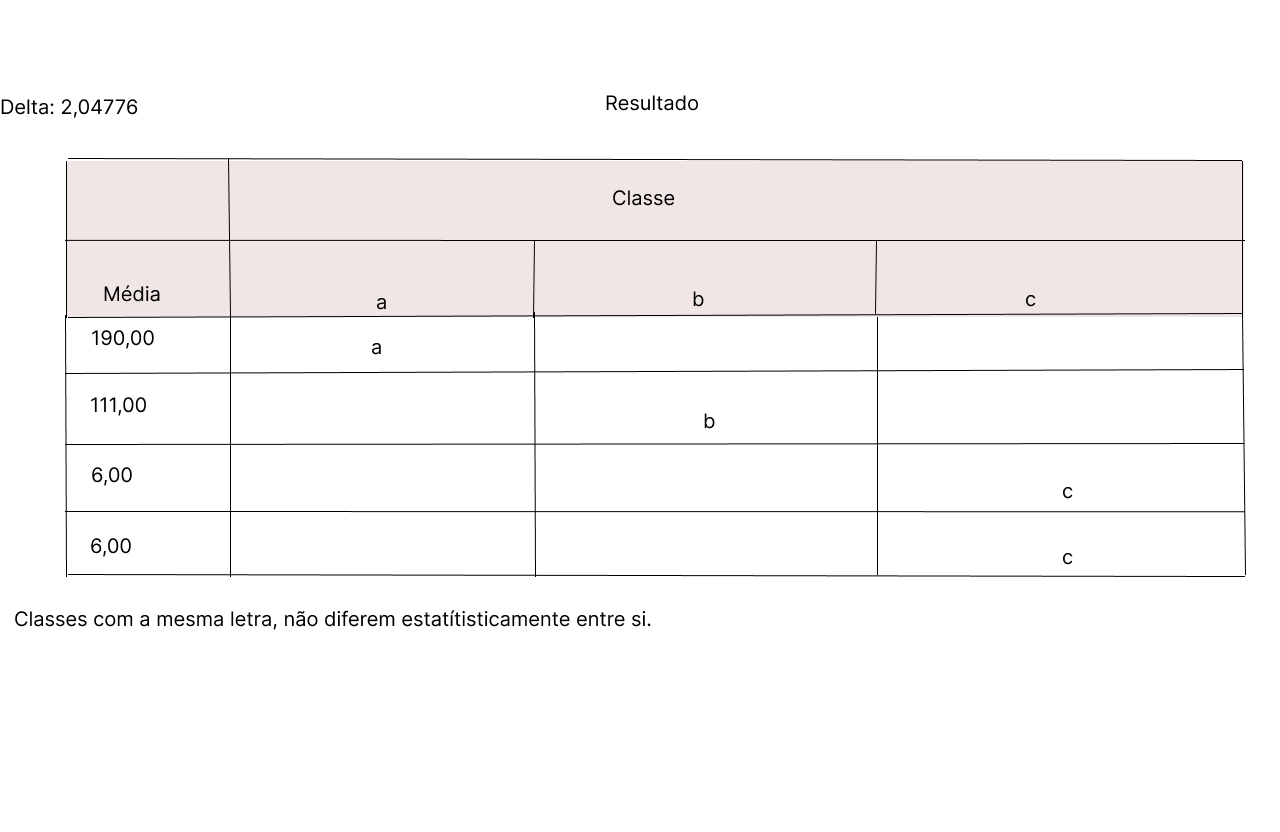
\includegraphics[width=0.8\linewidth]{imagens/tela2.png}
  \caption{Tela Resultado do Teste de Tukey}
  \label{fig:exemplo}
\end{figure}

\chapter{Implementação dos protótipos}
O código inclui a implementação dos protótipos das classes TesteTukey e TesteTukeyControle. Os métodos dentro dessas classes representam as operações necessárias para realizar o teste estatístico de Tukey em um conjunto de dados.


Classe TesteTukey
\begin{enumerate}
  \item Método temClasse e getNomeClasse: Esses métodos são usados para verificar se uma determinada classe está associada a uma média e obter o nome da classe com base em um índice.
  \item Método calcular: Este método realiza o cálculo principal do teste de Tukey, incluindo a ordenação das médias, o cálculo do delta e a classificação das médias em classes.
  \item Método calcularDelta: Calcula a diferença mínima significativa de Tukey com base nos parâmetros fornecidos.
  \item Método classificar: Este método classifica as médias em classes com base na diferença mínima significativa (delta).
\end{enumerate}


Classe TesteTukeyControle
\begin{enumerate}
  \item Método processar: Este método processa as ações solicitadas, como mostrar a configuração inicial ou calcular o teste de Tukey.
  \item Método mostrarConfiguracaoInicial e calcular: São responsáveis por exibir o formulário de entrada de dados e processar o cálculo do teste, respectivamente.
\end{enumerate}


HTML de Exibição de Resultados
\begin{enumerate}
  \item  Apresentação de Resultados: O código HTML é responsável por exibir os resultados do teste de Tukey, incluindo o valor de delta, uma tabela de médias classificadas em classes e uma mensagem explicativa sobre as classes.
\end{enumerate}

\begin{figure}[H]
  \centering
  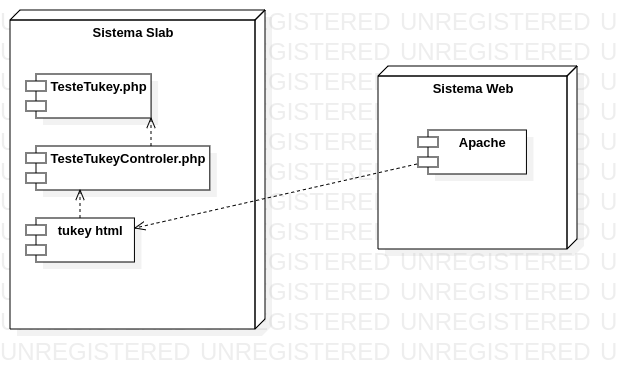
\includegraphics[width=0.8\linewidth]{imagens/componente.png} 
  \caption{Diagrama de Componente}
  \label{fig:exemplo}
\end{figure}

\chapter{Implantação dos protótipos}
\begin{figure}[H]
  \centering
  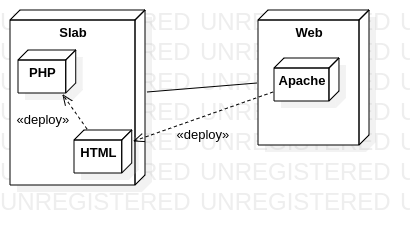
\includegraphics[width=0.8\linewidth]{imagens/implantação.png} 
  \caption{Diagrama de Implantação}
  \label{fig:exemplo}
\end{figure}